\chapter{Structures and Mechanisms}
\label{Chap: Structures}
\todo{definitions}
Now that the suspension length, number of cables, and attachment radius have been determined by the ADCS subsystem, a trade-off analysis for the gondola design can be initiated. In addition to these geometric constraints, subsystem-driven design preferences such as a high moment of inertia about the z-axis ($I_{zz}$), structural symmetry, and other performance drivers are taken into account. In this chapter ... \todo{finish intro}

\section{Requirements}
To ensure integrity of the overall structures design, several requirements are listed. These requirements contain all criteria the structure design must satisfy, and are given in \autoref{tab:struc_req}.

\todo{fill in TBD values}
\todo{ref REQ01 to entry and paper}

\begin{table}[H]
\centering
\caption{Structures requirements}
\label{tab:struc_req}
\begin{tabular}{ll}
\hline
\textbf{Requirement ID} & \textbf{Requirement} \\
\hline
REQ-STR-01 & The structure shall withstand all load cases corresponding to a maximum acceleration of 50 g during re-entry.\\
REQ-STR-02 & The aerobot and all supporting systems shall comply with the dimensional constraints imposed by the entry capsule. \\
REQ-STR-03 & The gondola mass shall not exceed 200 kg. \\
REQ-STR-04 & The structure shall withstand the TBD environmental loads. \\
REQ-STR-05 & The structural layout shall provide mounting provisions for two communication antennas positioned 180$^\circ$ apart. \\
REQ-STR-06 & The structural layout shall provide mounting provisions for two pyrgeometers aligned along a common axis, with one instrument facing upward and the other downward. \\
REQ-STR-07 & The structure shall supply a mechanism to connect the balloon tethers to the gondola. \\
REQ-STR-08 & The structural configuration shall not have any single-point failures. \\

\end{tabular}
\end{table}

\section{Design Option Tree}
For the gondola shape design, three options were considered: a sphere, cylinder and cuboid. An overview is given in \autoref{fig:STRUC_DOT}. From these options, the sphere was deemed as no viable option, according to the higher MMOI objective outlined in \autoref{chapter:ADCS}.

\begin{figure}
    \centering
    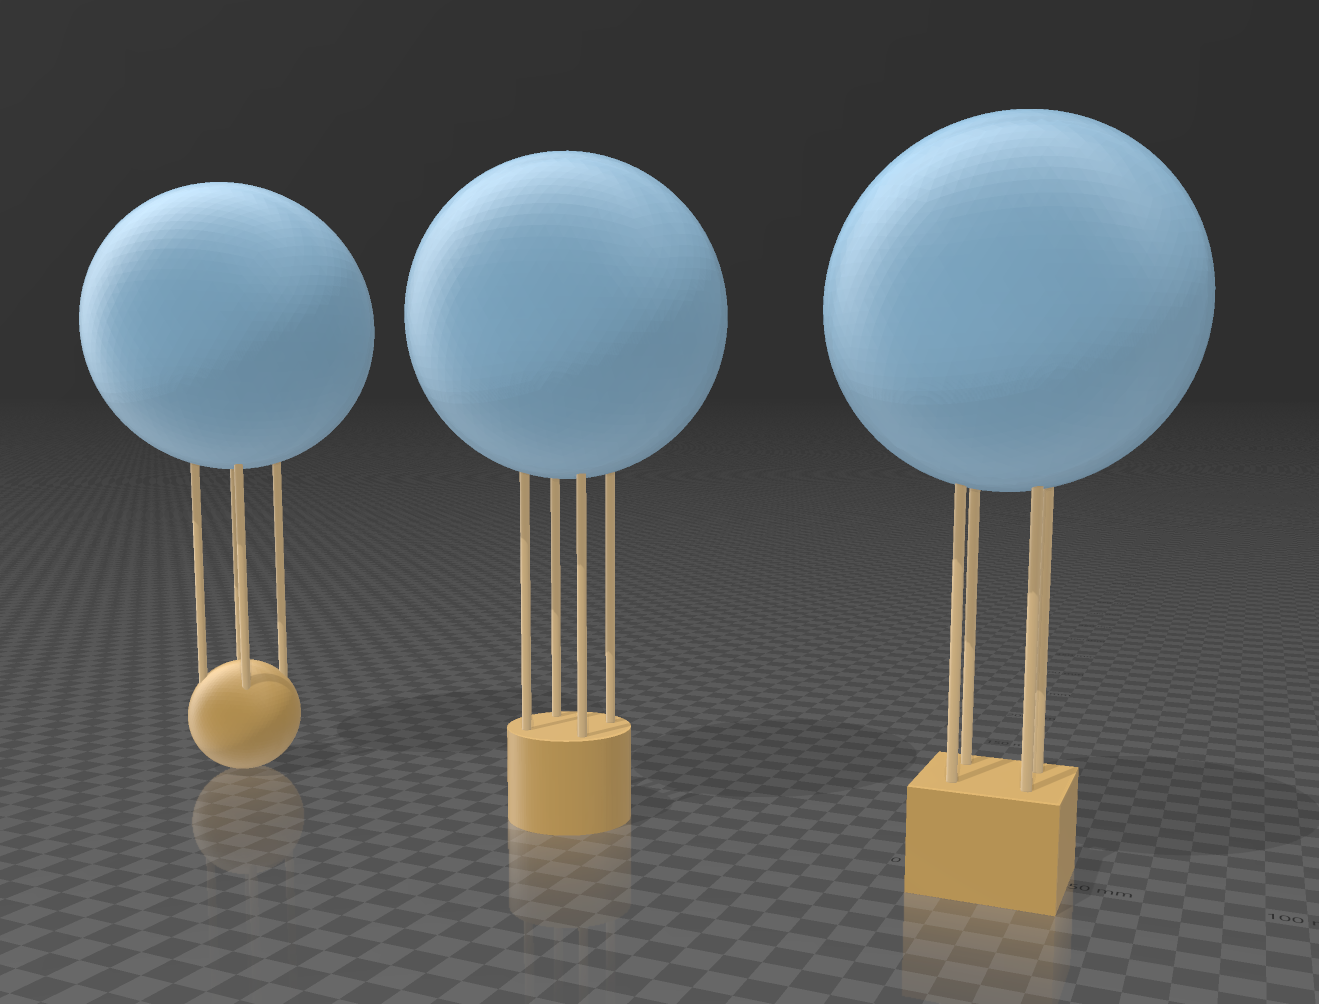
\includegraphics[width=0.5\linewidth]{fig/Gondola_Designs.PNG}
    \caption{The three considered gondola design options, not to scale.}
    \label{fig:STRUC_DOT}
\end{figure}

For the final trade-off for the gondola shape design, further analysis was necessary. For each of the options, their performance was graded upon various parameters. Aside from the requirements from \autoref{tab:struc_req}, additional parameters we considered. These consist of derived performance drivers, e.g. ADCS would benefit from a larger $I_{zz}$. An overview of all relevant drivers is given in \autoref{tab:struc_input1}.

\begin{table}[H]
\centering
\caption{Performance drivers from other subsystems, used as trade-off criteria between gondola shape options}
\label{tab:strc_input1}
\begin{tabular}{ll}
\hline
\textbf{Subsystem} & \textbf{Driver} \\
\hline
General & Minimize volume \\
General & Minimize complexity \\
ADCS & IMU placement close to c.g.\\
ADCS & Maximize MMOI about z-axis; $I_{zz}$\\
ADCS & Preserve symmetry about z-axis\\
Power & Sufficient surface area for solar panel placement $\geq 3900$ cm$^2$\\
Thermal & Minimize surface area\\
\end{tabular}
\end{table}

To begin the analysis, first, all components which needed to be placed inside the gondola were considered as cubes, with sizing based on their estimated volumes. Considering their requirements of orientation, and the parameters given in \autoref{tab:Struc_tradeoffcrit}, all components were laid out in both the cylinder and cuboid options. An overview of these layouts is given in \autoref{fig:struc_layouts}. 
\todo{fire CAD }
\begin{figure}[H]
    \centering

    \begin{subfigure}[b]{0.35\textwidth}
        \centering
        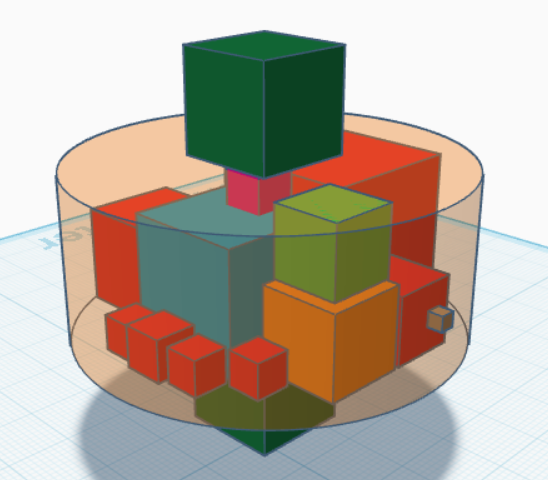
\includegraphics[width=\textwidth]{fig/STRUC_CYL.png}
        \caption{Cylindrical gondola configuration}
        \label{fig:cylinder_layout}
    \end{subfigure}
    \hfill
    \begin{subfigure}[b]{0.35\textwidth}
        \centering
        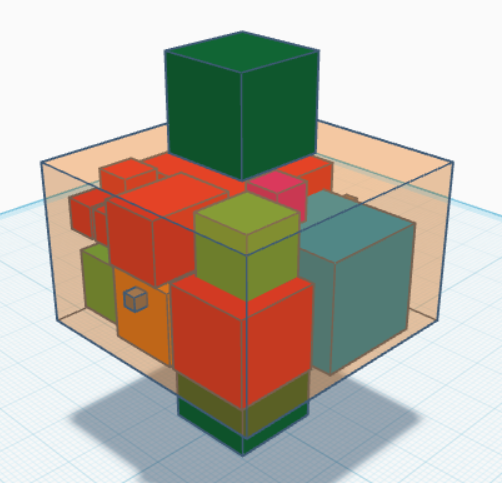
\includegraphics[width=\textwidth]{fig/STRUC_CUB.png}
        \caption{Cuboid gondola configuration}
        \label{fig:cuboid_layout}
    \end{subfigure}

    \caption{Preliminary internal layouts for the considered gondola configurations}
    \label{fig:struc_layouts}
\end{figure}

From these lay-outs, the preliminary estimations of the height, width, surface area and volume were derived for both options, as given in \autoref{tab:struc_est}. From these estimations, it can be seen that the cuboid gondola configuration yields the highest packing density, leading to the lowest surface area and volume. This however, does not directly give the mass and MMOI comparisons, as the thickness of each configurations still needs to be determined. This will be done in \autoref{sub:shell}. 

\subsection{Shell Configuration}\label{sub:shell}
The gondola shell was sized using a preliminary analogy-based sizing approach. The high-level shell design is anchored in comparable small-spacecraft structures that face similar constraints: compact geometry, strict mass limits, high quasi-static launch or entry accelerations. According to \textbf{Rajarajan 2021} and \textbf{Wills 2003} CubeSats and small-spacecraft references must comply with the 50g quasi-static structural load checks, aligned with those estimated in EDD. \textbf{Sekere 2017} CubeSat finite-element study using 2 mm aluminium faces motivates the shell thickness chosen for the VISTA mission. Furthermore, both \textbf{sekere 2017} and NASA SmallSat guidance identify aluminium 6061/7075 as the primary material for shell structures.

The selected baseline is therefore a reinforced gondola rather than a pure thin shell: a 2 mm coated aluminium alloy shell combined with internal ring frames, trays, and reinforced hard points. A simple average-stress check gives approximately $13.5~\mathrm{MPa}$ for the cylindrical shell and $14.2~\mathrm{MPa}$ for the cuboid shell, so global yielding is not the sizing driver. Instead, the 2 mm thickness is justified by local buckling, vibration and coating support. The final preliminary baseline is a cylindrical gondola with $R = 0.29~\mathrm{m}$, $h = 0.25~\mathrm{m}$, $t_{\mathrm{shell}} = 2~\mathrm{mm}$, a aluminium alloy shell/frame, and an estimated shell mass of approximately $5.3~\mathrm{kg}$. The cuboid option, with dimensions $0.43 \times 0.43 \times 0.27~\mathrm{m}$, $t_{\mathrm{shell}} = 2~\mathrm{mm}$, and shell mass of approximately $4.5~\mathrm{kg}$, is retained as a backup in case packaging or mass-budget conflicts emerge. However, the cylinder is preferred due to its symmetry, cleaner inertia properties, lower ADCS coupling risk, larger volume, and structurally efficient curvature.

\subsection{Suspension Cables}
The suspension cable selection was performed as a preliminary trade-off between polymer fibre ropes and metallic cable alternatives, using tensile capacity, mass, cost, environmental robustness and creep/degradation risk as the main criteria.  Three feasible configurations were therefore retained: Vectran/LCP rope with protective jacket/coating, aramid rope with protective jacket, and coated titanium cable. The metallic option is mechanically robust but heavier and still requires environmental protection, while aramid is lightweight but less attractive due to long-term degradation and creep concerns. Vectran/LCP provides the best balance of low mass, high tensile strength, low creep, and existing high-performance rope heritage. The protective layer is assumed to be a fluoropolymer-based coating/jacket, such as PTFE/FEP-type protection, to limit direct exposure of the fibres to sulfuric acid aerosols, UV, thermal cycling, abrasion, and handling damage.

For the current four-cable suspension, each cable is $15 m$ long, giving $60 m$ total cable length. A $4 mm$ Vectran/LCP rope is selected as the preliminary baseline, with an estimated bare rope density of $10g/m$. Hence, the mass of the suspension cables, combined with that of the $300 m$ tether (Payload), the bare rope would weigh $3.6 kg$, and a conservative full cable-package mass of about $5 kg$, including terminations and protection jackets. The expected maximum cable load is approximately $200 N$ per cable, while a conservative safety factor of 10 is applied to account for harsh-environment degradation, creep, coating/jacket damage and other losses. Even with this conservative factor, the design load remains well below the breaking load of a representative $4 mm$ Vectran/LCP rope, which is on the order of $10–15 kN$. Therefore, the cable selection is not strength-limited; the main design drivers are environmental protection, long-duration material stability, termination reliability, and maintaining the protective fluoropolymer coating/jacket throughout the mission. \todo[inline]{\textbf{add references!!!!!}}


    \begin{itemize}
        \item balloon 
        \item hoop stress etc.
        \item skeleton?
    \end{itemize}

\section{Verification Plan}
To verify that the structure will satisfy all given requirements, a verification plan must be established. For each items, an appropriate methods need to be chosen. An overview of these items with corresponding methods is given in \autoref{tab:struc_vnv}.

\begin{table}[H]
\centering
\caption{Verification items and associated verification methods for the structural verification plan}
\label{tab:struc_vnv}
\begin{tabular}{ll}
\hline
\textbf{Item} & \textbf{Verification Method} \\
\hline
Structural mass & Mass properties extracted from CAD model and material property data \\
Geometric constraints & CAD-based envelope compliance assessment against entry capsule interface \\
Load capacity (50 g) & Equivalent static load case analysis supported by analytical calculations \\
Cable safety factor ($SF=10$) & Analytical tension analysis under worst-case loading conditions \\
Hard-point strength & Stress analysis using analytical methods and finite element analysis \\
Global structural stiffness & Simplified analytical model supported by FEM validation \\
Local buckling resistance & Buckling analysis of critical structural elements \\
IMU mounting stiffness & Local stiffness evaluation supported by simplified modal assessment \\
Thermal compatibility & Material and coating selection based on environmental compatibility assessment \\
\hline
\end{tabular}
\end{table}

\section{Mass Budget}
Now that all components have been selected regarding every subsystem, a preliminary mass budget can be made to estimate the total mass. In this analysis, all components were considered, including a margin to account for uncertainties. These margins were based on the maturity, level of confidence and potential design changes of each system. The mass budget overview is given in \autoref{tab:mass_budget}.

\begin{longtable}{llrrrr}
\caption{Cleaned subsystem mass budget} \\
\hline
\textbf{Subsystem} & \textbf{Component} & \textbf{\#} & \textbf{Mass (kg)} & \textbf{Margin} & \textbf{Total mass incl. margin (kg)} \\
\hline
\endfirsthead

\hline
\textbf{Subsystem} & \textbf{Component} & \textbf{\#} & \textbf{Mass (kg)} & \textbf{Margin} & \textbf{Total mass (kg)} \\
\hline
\endhead

ADCS & IMU & 1 & 0.500 & 10\% & 0.550 \\
CDHS & All except computer & 1 & 0.300 & 10\% & 0.330 \\
\hline

ISRU & Valves & 3 & 0.014 & 20\% & 0.051 \\
ISRU & Pump/Intake & 1 & 0.550 & 20\% & 0.660 \\
ISRU & N2 Storage Tank & 1 & 0.180 & 20\% & 0.216 \\
ISRU & Controller Unit & 1 & 0.076 & 20\% & 0.091 \\
ISRU & N2 Separator & 1 & 0.300 & 20\% & 0.360 \\
ISRU & N2 Pump & 1 & 0.250 & 20\% & 0.300 \\
ISRU & Pressure Sensors & 2 & 0.220 & 20\% & 0.528 \\
\hline

PAY & Mass Spectrometer & 1 & 10.900 & 10\% & 11.990 \\
PAY & Nephelometer & 1 & 0.800 & 10\% & 0.880 \\
PAY & Laser Spectrometer & 1 & 0.620 & 10\% & 0.682 \\
PAY & pH Sensor & 1 & 0.350 & 10\% & 0.385 \\
PAY & Weather Instrument Suite & 1 & 0.100 & 10\% & 0.110 \\
PAY & Pyrgeometer & 2 & 1.300 & 10\% & 2.860 \\
PAY & Sonic Anemometer & 1 & 0.400 & 10\% & 0.440 \\
PAY & Optical Particle Counter & 1 & 2.000 & 10\% & 2.200 \\
PAY & Barometer & 5 & 0.050 & 10\% & 0.275 \\
\hline

TCS & Cooling system & 1 & 5.000 & 20\% & 6.000 \\
TCS & Heating system & 1 & 1.000 & 20\% & 1.200 \\
TCS & Temp. sensors & 15 & 0.004 & 20\% & 0.072 \\
\hline

STRUC & Barometer tether & 1 & 4.160 & 40\% & 5.824 \\
STRUC & Tether reel/motor & 1 & 2.000 & 40\% & 2.800 \\
STRUC & Balloon tethers & 4 & 0.200 & 40\% & 1.120 \\
STRUC & Gondola structure & 1 & 5.000 & 40\% & 7.000 \\
\hline

PWR & Solar panels & 1 & 3.000 & 20\% & 3.600 \\
PWR & Battery & 1 & 4.000 & 20\% & 4.800 \\
PWR & PCDU & 1 & 1.500 & 20\% & 1.800 \\
\hline

COM & HRA & 1 & 0.120 & 10\% & 0.132 \\
COM & UHF & 1 & 0.037 & 10\% & 0.041 \\
COM & Other hardware & 1 & 0.080 & 10\% & 0.088 \\
\hline

TTC & X-band transponder & 1 & 3.000 & 10\% & 3.300 \\
TTC & Antenna & 1 & 1.000 & 10\% & 1.100 \\
\hline

\textbf{TOTAL} &  &  & \textbf{49.011} &  & \textbf{61.785} \\
\hline
\end{longtable}

\todo{ref deployment}
Including the margins, the total mass is estimated to be 71.1 kg. It should be noted that this excludes the mass of the deployment stage, as given in \autoref{XX}. In this budget, a significant margin for the structures and mechanism subsystem is given, due to the additional load carrying structures, which are not identified fully yet. 

% TOTAL TABLE (IN CONCLUSION SECTION?)
\begin{table}[H]
\centering
\caption{Parameters derived from gondola lay-out}
\label{tab:struc_est}
\begin{tabular}{lll}
\hline
\textbf{Parameter} & \textbf{Cylinder} & \textbf{Cuboid} \\
\hline
Height (cm) & 25 & 27 \\
Width/Diameter (cm) & 58 & 43 \\
Surface area (cm$^2$) & 9840 & 8342 \\
Volume (cm$^3$) & 66070 & 49923 \\
Thickness (cm) & 0.2 & 0.2 \\
Mass (kg) & 5.3 & 4.5 \\
% Moment of Inertia (kg$\cdot$m$^2$) & & \\
\end{tabular}
\end{table}

